\documentclass[UTF8]{ctexbeamer}

\usetheme{Pittsburgh}
\usefonttheme[onlymath]{serif}

\usepackage{subfig}
\usepackage{multirow}
\usepackage{xcolor,colortbl}
\usepackage{listings}
\usepackage{amsmath}

% Solarized colors
\definecolor{sbase03}{HTML}{002B36}
\definecolor{sbase02}{HTML}{073642}
\definecolor{sbase01}{HTML}{586E75}
\definecolor{sbase00}{HTML}{657B83}
\definecolor{sbase0}{HTML}{839496}
\definecolor{sbase1}{HTML}{93A1A1}
\definecolor{sbase2}{HTML}{EEE8D5}
\definecolor{sbase3}{HTML}{FDF6E3}
\definecolor{syellow}{HTML}{B58900}
\definecolor{sorange}{HTML}{CB4B16}
\definecolor{sred}{HTML}{DC322F}
\definecolor{smagenta}{HTML}{D33682}
\definecolor{sviolet}{HTML}{6C71C4}
\definecolor{sblue}{HTML}{268BD2}
\definecolor{scyan}{HTML}{2AA198}
\definecolor{sgreen}{HTML}{859900}

\lstset{
    % How/what to match
    sensitive=true,
    % Border (above and below)
    frame=lines,
    % Extra margin on line (align with paragraph)
    xleftmargin=\parindent,
    % Put extra space under caption
    belowcaptionskip=1\baselineskip,
    % Colors
    backgroundcolor=\color{sbase3},
    basicstyle=\color{sbase00}\ttfamily,
    keywordstyle=\color{scyan},
    commentstyle=\color{sbase1},
    stringstyle=\color{sblue},
    numberstyle=\color{sviolet},
    identifierstyle=\color{sbase00},
    % Break long lines into multiple lines?
    breaklines=true,
    % Show a character for spaces?
    showstringspaces=false,
    tabsize=2
}


% Title
\title{第10章 函数图表构成模型}
\author{韩建伟}
\institute{
  浙江工商大学信息学院\\
  \texttt{hanjianwei@mail.zjgsu.edu.cn}
}
\date{2011/12/05}

\begin{document}

% Title page
\begin{frame}[plain]
  \titlepage{}
\end{frame}

\begin{frame}{军备竞赛}
  
  \begin{block}{两种战略}
    \begin{description}
    \item[友好战略] 在第一次大规模打击之后生存下来,并且给予敌人无法承受的回击
    \item[敌对战略] 第一次就进行大规模的打击,摧毁对方的导弹力量
    \end{description}    
  \end{block}

  
  \begin{block}{核威慑策略} 
    \begin{itemize}
    \item 在确定自己的导弹力量时奉行友好战略
    \item 假设对方实行敌对战略
    \end{itemize}
  \end{block}
  
\end{frame}

\begin{frame}{变量定义}
  \begin{itemize}
  \item $x$:国家$X$拥有的导弹数量
  \item $y$: 国家$Y$拥有的导弹数量
  \item $x=g(y)$: $X$为实现它的战略所需要的最低导弹数
  \item $y=f(x)$: $Y$为实现它的战略所需要的最低导弹数
  \item $x_0$: $X$为摧毁$Y$的人口和工业中心所需的导弹数
  \item $y_0$: $Y$为摧毁$X$的人口和工业中心所需的导弹数
  \end{itemize}
\end{frame}

\begin{frame}{国家$Y$的策略}
  \begin{itemize}
  \item 心理防卫:即使$X$没有导弹,$Y$也要$y_0$枚导弹
  \item 武器技术限制:$X$每发射一枚导弹只能摧毁$Y$不多于一枚的导弹
  \item $X$每增加一枚导弹,$Y$需增加的导弹取决于$X$导弹的效率
  \end{itemize}
  
  \begin{figure}
    \centering
    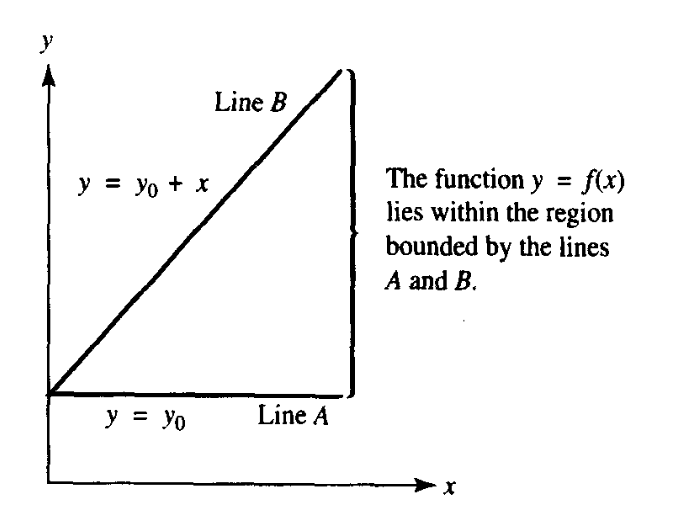
\includegraphics[width=0.6\textwidth]{region.png}
  \end{figure}
\end{frame}

\begin{frame}{分情况讨论}
  \begin{itemize}
  \item 根据两国的导弹数量将A和B之间的区域分成几个子区域
  \end{itemize}
  
  \begin{figure}
    \centering
    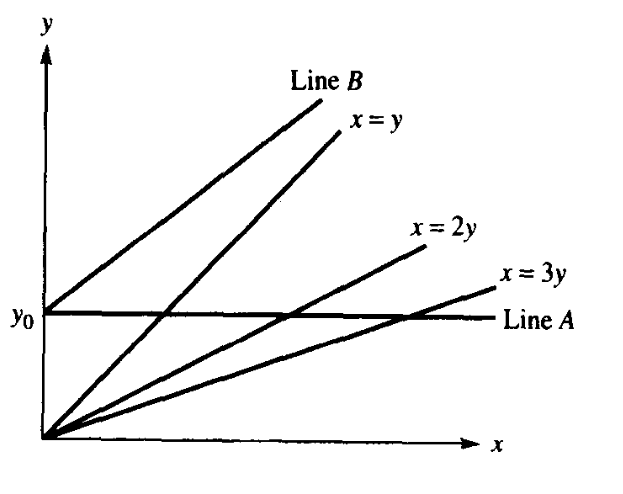
\includegraphics[width=0.6\textwidth]{case.png}
  \end{figure}
\end{frame}

\begin{frame}{情况1: $x < y$}
  \begin{itemize}
  \item $X$发射的$x$枚导弹攻击$Y$相同数量的导弹
  \item $s$表示$Y$受到攻击导弹的幸存率
  \end{itemize}
  \[
  \begin{array}{cc}
    y_0 = y - x + sx, & 0 < s < 1
  \end{array}
  \]
  或者
  \[
  \begin{array}{cc}
    y = y_0 +(1-s)x, & 0 < s < 1
  \end{array}
  \]
\end{frame}

\begin{frame}{情况2: $y = x$}
  \begin{itemize}
  \item $X$用自己的每一枚导弹瞄准$Y$的每一枚导弹
  \item 幸存的导弹为$sx = sy$
  \end{itemize}

  \[
  y = \frac{y_0}{s}
  \]
  
\end{frame}

\begin{frame}{情况3: $y < x < 2y$}
  \begin{itemize}
  \item $X$在发射它的导弹时,瞄准$Y$的每一枚导弹一次,部分两次
  \item $x-y$枚导弹被瞄准两次,剩余$s^2(x-y)$
  \item $y-(x-y) = 2y-x$枚导弹被瞄准一次,剩余$s(2y-x)$
  \end{itemize}
  
  \begin{figure}
    \centering
    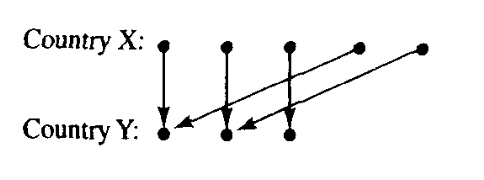
\includegraphics[width=0.4\textwidth]{neardouble.png}
  \end{figure}
  
  \[
  y_0 = s^2(x-y) + s(2y-x)
  \]
  故
  \[
  y = \frac{y_0 + x(s-s^2)}{2s - s^2}
  \]
\end{frame}

\begin{frame}{情况4:$x=2y$}
  \begin{itemize}
  \item $X$用两枚导弹瞄准$Y$的一枚导弹,剩余$s^2y$导弹
  \end{itemize}
  \[
  y = \frac{y_0}{s^2}
  \]

\end{frame}

\begin{frame}{分段表示}

  \begin{figure}
    \begin{minipage}{.5\linewidth}
      \[
      y =
      \left\{
        \begin{array}{ll}
          y_0 +(1-s)x, & x < y\\
          \frac{y_0}{s}, & x = y\\
          \frac{y_0 + x(s-s^2)}{2s - s^2}, & y < x < 2y\\
          \frac{y_0}{s^2},& x = 2y
        \end{array}
      \right.
      \]
    \end{minipage}%
    \begin{minipage}{.5\linewidth}
      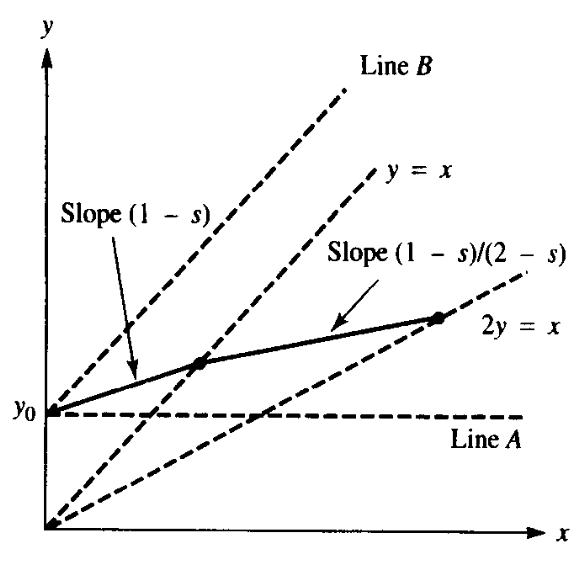
\includegraphics[width=.8\textwidth]{linear.png}
    \end{minipage}
  \end{figure}

  \begin{itemize}
  \item 交点: $(0, y_0)$, $(x, x)$, $(x, \frac{x}{2})$, $(x, \frac{x}{3})$, ...
  \item $y$值:$\frac{y_0}{s}$, $\frac{y_0}{s^2}$, ...
  \end{itemize}

\end{frame}

\begin{frame}{连续形式}
  \begin{itemize}
  \item 推广到连续形式:
  \end{itemize}
  \[
  \begin{array}{ll}
    y = \frac{y_0}{s^{x/y}}, & 0 < s < 1
  \end{array}
  \]
  
  \begin{figure}
    \centering
    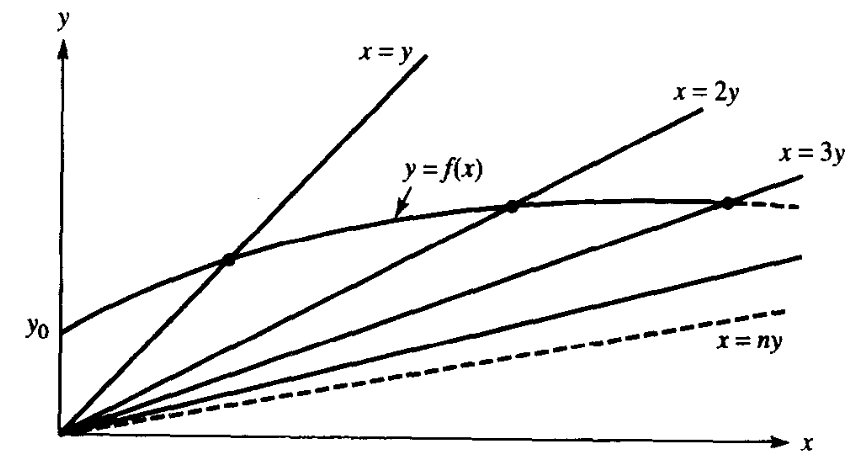
\includegraphics[width=.6\textwidth]{continue.png}
  \end{figure}
\end{frame}

\begin{frame}{同时考虑$X$, $Y$}
  \begin{itemize}
  \item 黑色区域:双方都满意的区域
  \item $(x_m, y_m)$:双方都能满意的最少导弹数量
  \item 双方导弹数如何变化?
  \end{itemize}
  
  \begin{figure}
    \centering
    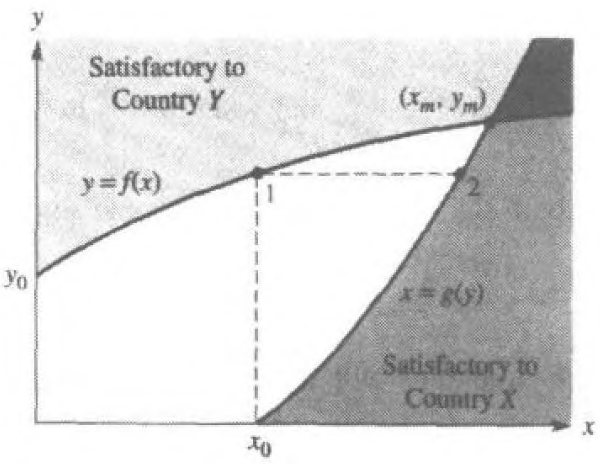
\includegraphics[width=.5\textwidth]{two.png}
  \end{figure}

\end{frame}

\begin{frame}{交点的唯一性}
  \begin{itemize}
  \item $y=f(x)$, $x=g(y)$都是增函数
  \item 如果两者有多个交点,则其二阶导数改变符号
  \item 证明$f(x)$的二阶导总是负的
  \end{itemize}

  \begin{figure}
    \centering
    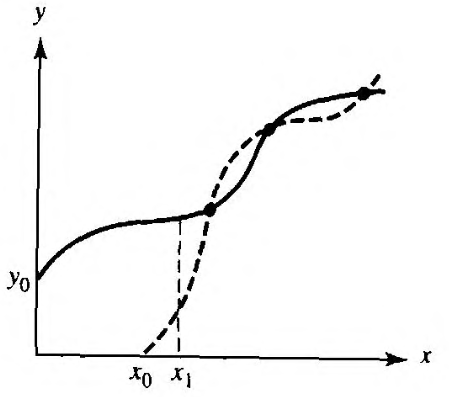
\includegraphics[width=.5\textwidth]{neg.png}
  \end{figure}
  
\end{frame}

\begin{frame}{函数$y=f(x)$的图形行为}

  \begin{figure}
    \centering
    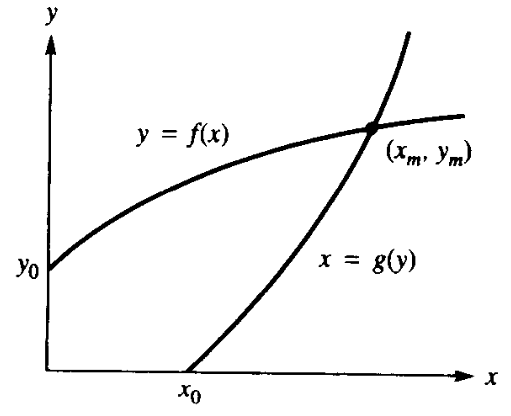
\includegraphics[width=.4\textwidth]{model.png}
  \end{figure}
  
  \begin{itemize}
  \item 最低导弹数$y_0$
  \item 保全百分比$s$
  \item 交换比值$e = \frac{x}{y}$
  \item 对于$x=g(y)$有类似的变量
  \item 当这些因素变化时,$(x_m, y_m)$如何变化?
  \end{itemize}
  
\end{frame}

\begin{frame}{城市防御}
  \begin{itemize}
  \item 假设$X$将其民防预算增加一倍
  \item $y_0\uparrow$, 其它值都不变
  \item 效果:$y=f(x)$上移并且每一个$x$处斜率增大
  \item 新交点$(x'_m, y'_m)$, $x'_m > x_m$, $y'_m > y_m$
  \end{itemize}

  \begin{figure}
    \centering
    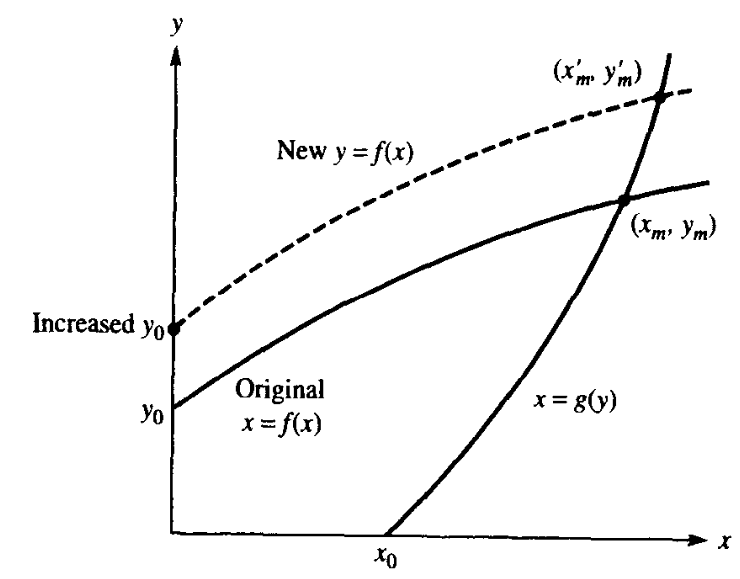
\includegraphics[width=.5\textwidth]{cd.png}
  \end{figure}
  
\end{frame}

\begin{frame}{移动发射台}
  \begin{itemize}
  \item $X$将其导弹放在移动发射台上
  \item $s\uparrow$, 其它值保持不变
  \item 效果: 把$x=g(y)$向上拉直
  \item 新交点$(x'_m, y'_m)$, $x'_m < x_m$, $y'_m < y_m$
  \end{itemize}

  \begin{figure}
    \centering
    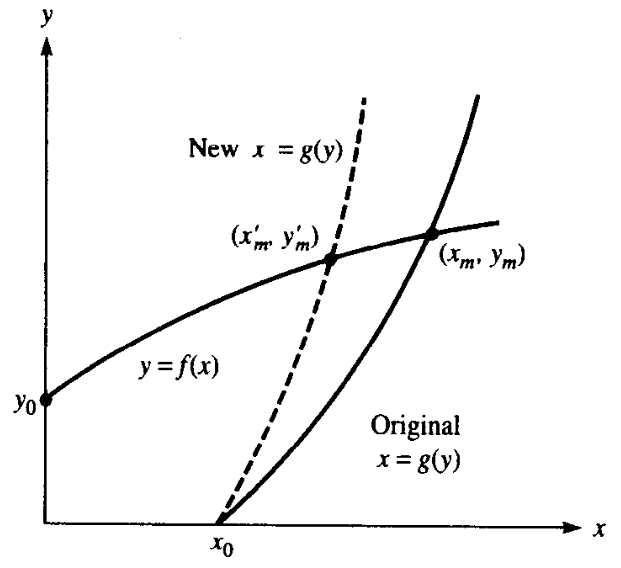
\includegraphics[width=.45\textwidth]{ml.png}
  \end{figure}

\end{frame}

\begin{frame}{多弹头}
  \begin{itemize}
  \item 假设每枚导弹装载多个弹头
  \item $x_0$, $y_0$下降
  \item 当$X$的导弹增加时,$Y$的导弹极具增加
  \item 效果: 截距减小,但是斜率增加
  \item 新交点$(x'_m, y'_m)$, 与原交点$(x_m, y_m)$的关系不一定
  \end{itemize}

  \begin{figure}
    \centering
    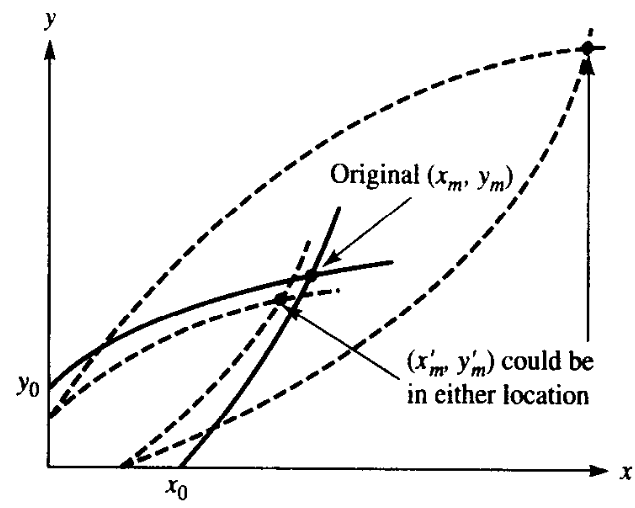
\includegraphics[width=.45\textwidth]{mw.png}
  \end{figure}
  
\end{frame}

\begin{frame}{多弹头:弹头计数}
  \begin{itemize}
  \item 按照弹头的个数进行分析
  \item $x_0$, $y_0$不变,现在一枚弹头就可以摧毁$Y$的16个弹头,因此交换比例大大增加
  \item 效果: 曲线变陡
  \item 新交点$(x'_m, y'_m)$, $x'_m > x_m$, $y'_m > y_m$
  \end{itemize}

  \begin{figure}
    \centering
    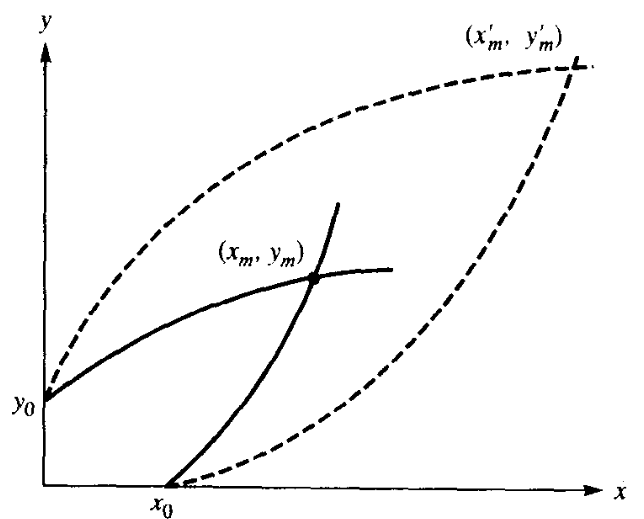
\includegraphics[width=.45\textwidth]{wc.png}
  \end{figure}
  
\end{frame}

\begin{frame}{对分阶段军备竞赛建立模型}
  \begin{block}{威慑战略}
    \begin{itemize}
    \item 自身拥有一定数量的武器来威慑敌人,即使对方根本没有武器
    \item 随着敌人增加武器,会按照其攻击武器的某个百分比提高军备投资
    \end{itemize}
  \end{block}
  \begin{itemize}
  \item $y = 120 + \frac{1}{2}x$
  \item $x = 60 + \frac{1}{3}y$
  \end{itemize}

\end{frame}

\begin{frame}{一种图表解法}
  \begin{table}
    \centering
    \begin{tabular}{c|cccccc}
      阶段$n$ & 0 & 1 & 2 & 3 & 4 & 5\\
      \hline
      国家$Y$ & 0 & 120 & 150 & 170 & 175 & 178\\
      国家$X$ & 0 & 60 & 100 & 110 & 117 & 118
    \end{tabular}
  \end{table}

  \begin{figure}
    \centering
    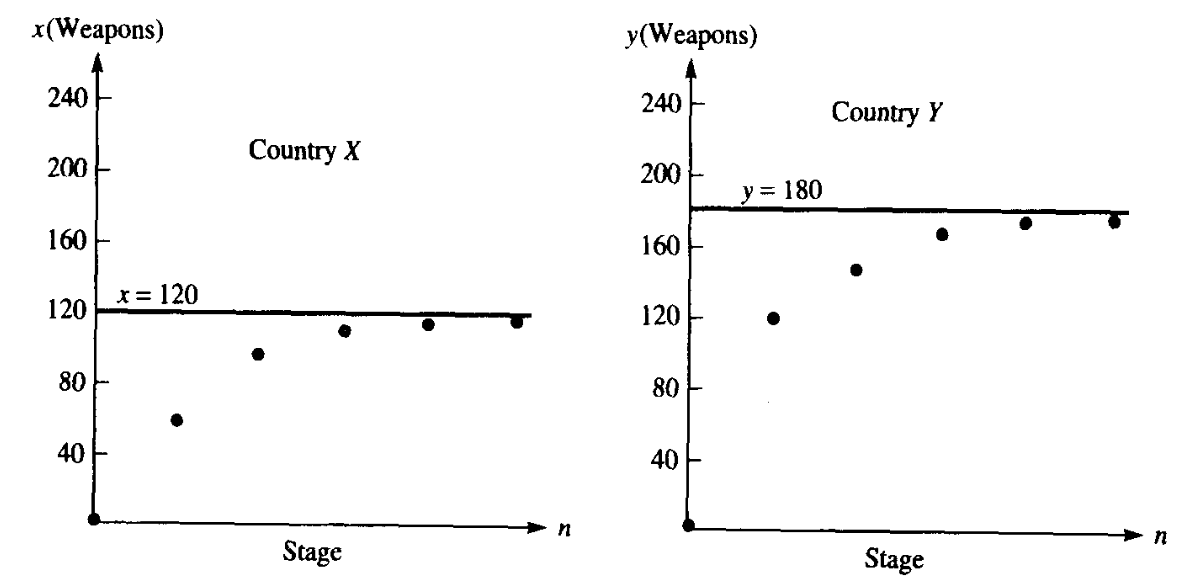
\includegraphics[width=.7\textwidth]{dar.png}
  \end{figure}
  
\end{frame}

\begin{frame}{数值解}
  \begin{figure}
    \begin{minipage}{.5\linewidth}
      \[
      \left.
        \begin{array}{l}
          y_{n+1}=120 + \frac{1}{2}x_n\\
          x_{n+1}=60 + \frac{1}{3}y_n\\
          x_0 = 0\\
          y_0 = 0
        \end{array}
      \right\}
      \]
    \end{minipage}%
    \begin{minipage}{.5\linewidth}
      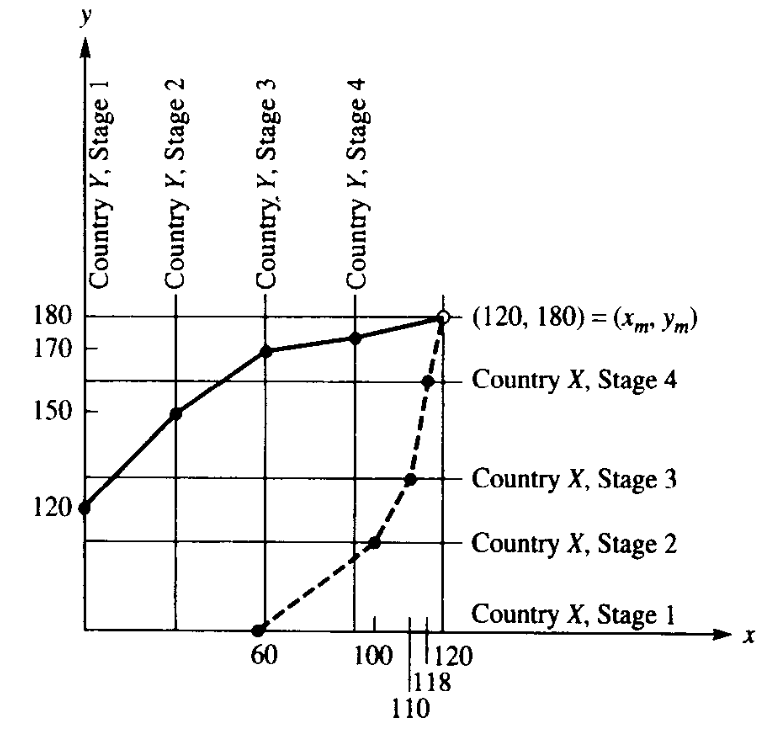
\includegraphics[width=\textwidth]{arc.png}
    \end{minipage}
  \end{figure}

  \begin{itemize}
  \item 如果$x_0=100, y_0=120$呢?
  \end{itemize}

\end{frame}

\begin{frame}{能源危机}
  \begin{itemize}
  \item 附加税对于短期和长期消费者需求的影响是什么?
  \item 谁在实际缴纳附加税——消费者还是公司?
  \item 附加税促使通货膨胀么?
  \end{itemize}
\end{frame}

\begin{frame}{构造一个图表模型}
  \begin{itemize}
  \item 如何确定公司的最佳利润$q^*$
  \item $TP = TR - TC \Rightarrow TP' = TR' - TC' = 0 \Rightarrow TR'(q^*) = TC'(q^*)$
  \item $TR'(q) \approx \frac{TR(q+\Delta q)-TR(q)}{\Delta q}$,
  \item 边际收益:如果$\Delta q = 1$,则$TR'(q) \approx TR(q+1)-T(q)=M(q)$
  \item 最大利润$q^*$的必要条件: $MR(q^*) = MC(q^*)$
  \item 解释...
  \end{itemize}
  
  \begin{figure}
    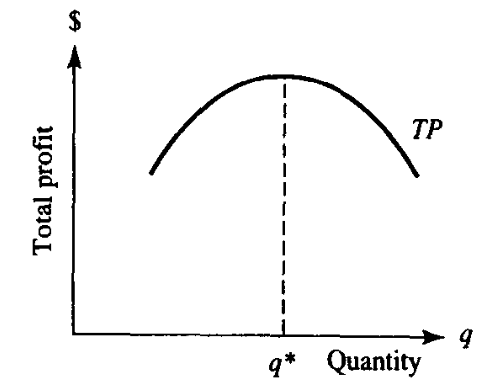
\includegraphics[height=.35\textheight]{profit.png}
    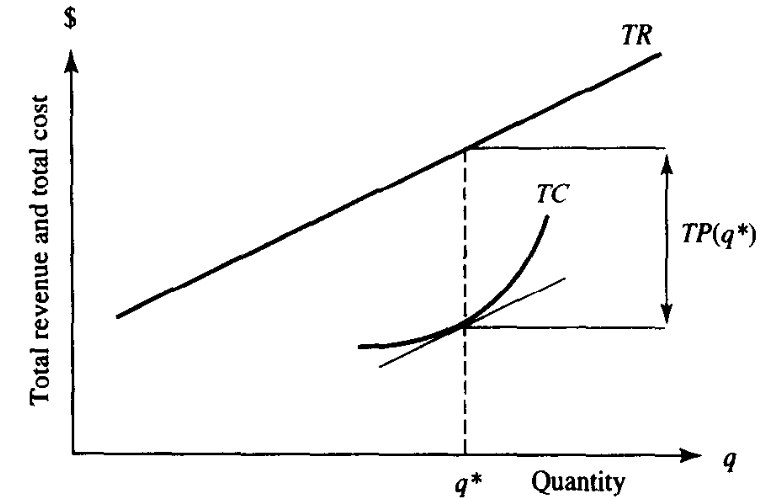
\includegraphics[height=.35\textheight]{totalcr.png}
    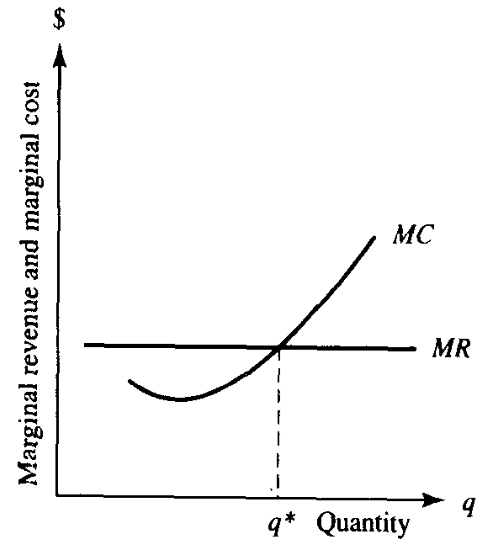
\includegraphics[height=.35\textheight]{mcr.png}
  \end{figure}

\end{frame}

\begin{frame}{税收对于能源危机的影响}
  \begin{itemize}
  \item 政府增加税收
  \item 公司通过提高价格抵消税收
  \item 结果:导致通货膨胀,石油数量未减少
  \end{itemize}

  \begin{figure}
    \centering
    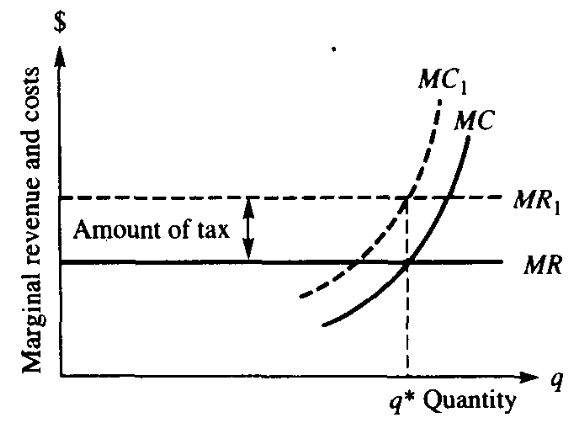
\includegraphics[width=.5\textwidth]{taxshift.png}
  \end{figure}

\end{frame}

\begin{frame}{公司对价格的反应}

  \begin{itemize}
  \item 市场价格升高,企业乐于生产更大数量的产品
  \end{itemize}
  
  \begin{figure}
    \centering
    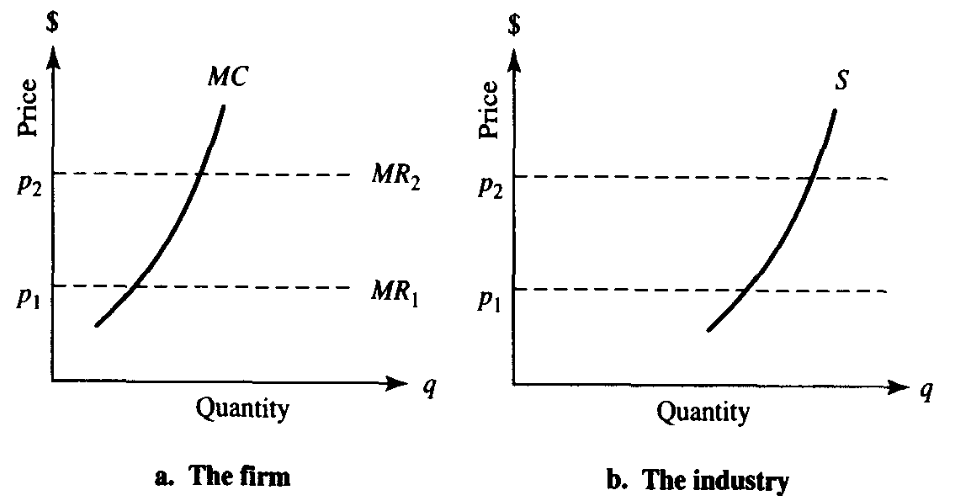
\includegraphics[width=.7\textwidth]{ap.png}
  \end{figure}

\end{frame}

\begin{frame}{消费者对于价格的反应}

  \begin{itemize}
  \item 市场价格升高,消费者较少使用或者转用更便宜的替代品
  \end{itemize}

  \begin{figure}
    \centering
    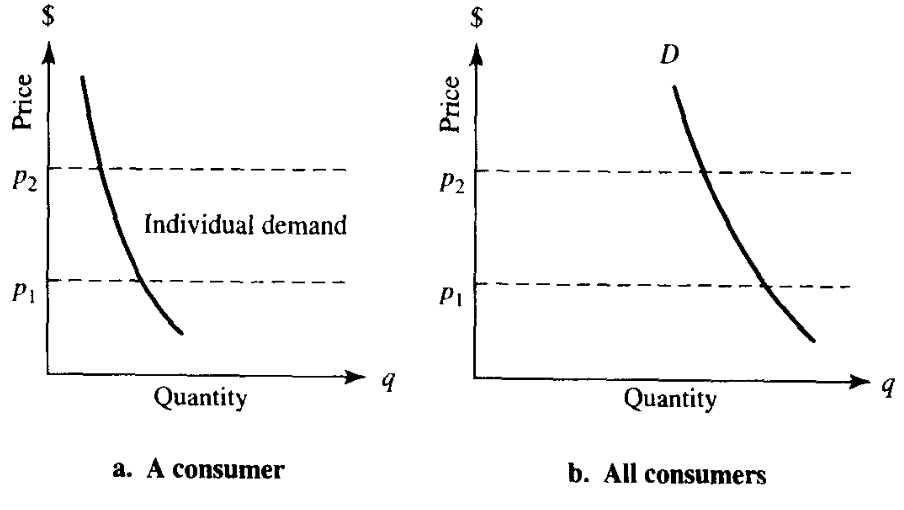
\includegraphics[width=.7\textwidth]{cp.png}
  \end{figure}
  
\end{frame}

\begin{frame}{综合考虑}
  \begin{itemize}
  \item $(q^*, p^*)$使消费者和公司都满意
  \end{itemize}

  \begin{figure}
    \centering
    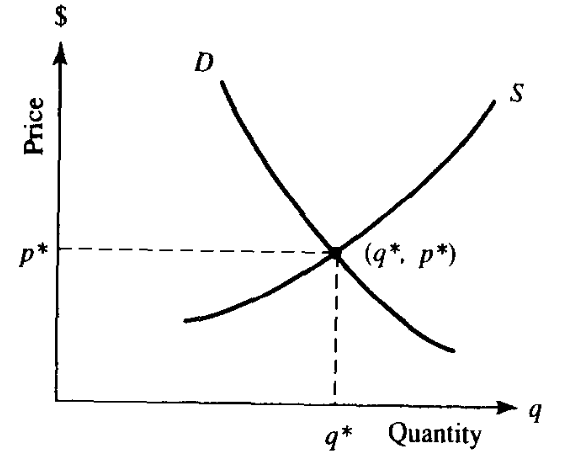
\includegraphics[width=.5\textwidth]{both.png}
  \end{figure}
  
\end{frame}

\begin{frame}{如果没有位于$q^*$会如何?}
  \begin{itemize}
  \item 供应比需求曲线陡峭:最终达到平衡
  \item 需求比供应曲线陡峭:平衡点难以达到
  \end{itemize}

  \begin{figure}
    \centering
    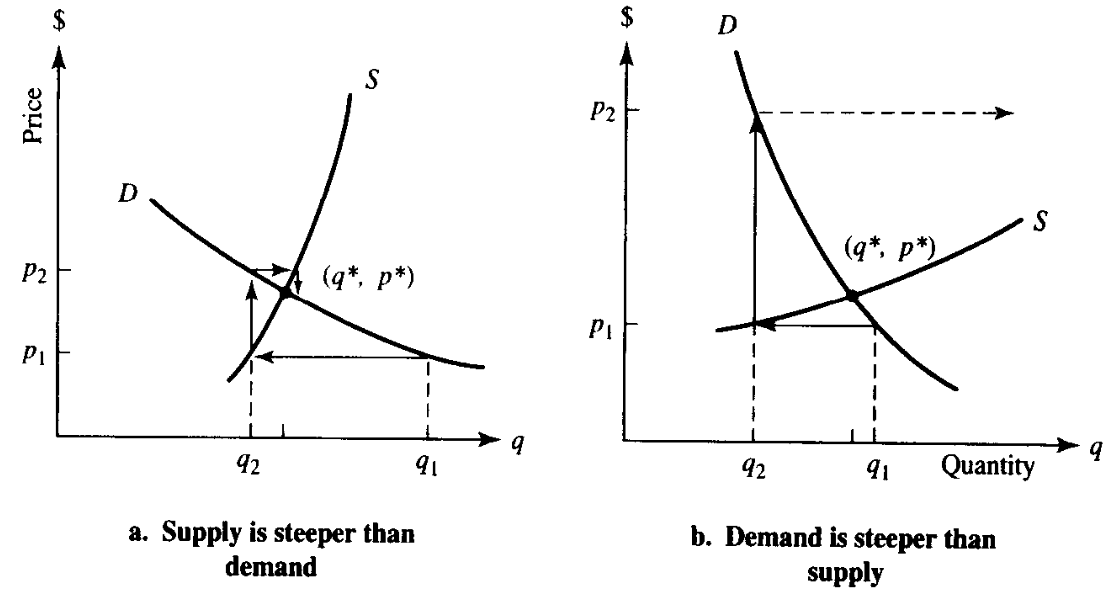
\includegraphics[width=.7\textwidth]{sd.png}
  \end{figure}

\end{frame}

\begin{frame}{考虑税收}
  \begin{itemize}
  \item 成本曲线向上移动税款量那么多
  \item 价格上升低于税款,说明公司和消费者分摊税款
  \item 产品数量下降
  \end{itemize}

  \begin{figure}
    \centering
    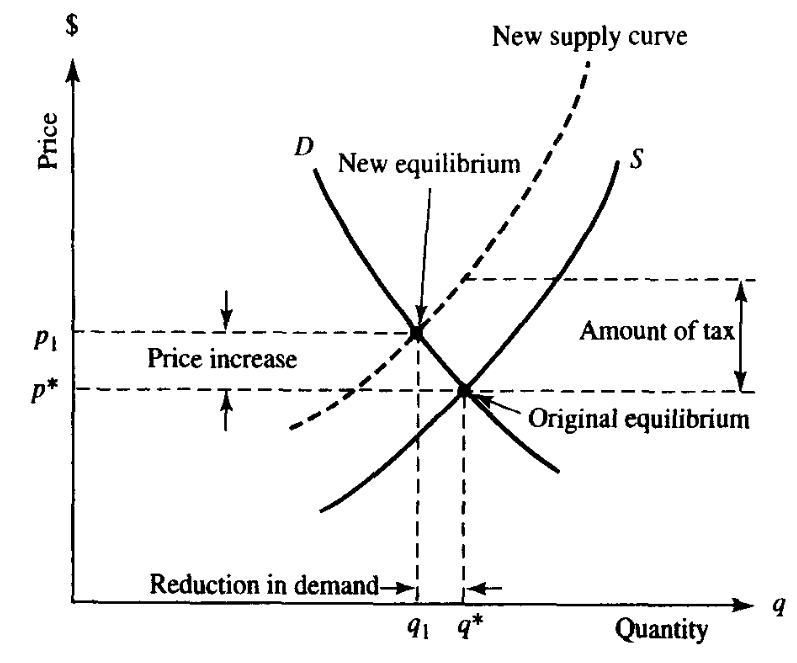
\includegraphics[width=.5\textwidth]{tax.png}
  \end{figure}
  
\end{frame}

\begin{frame}{石油短缺}
  \begin{itemize}
  \item 短期内,石油企业对于价格更加敏感
  \end{itemize}

  \begin{figure}
    \centering
    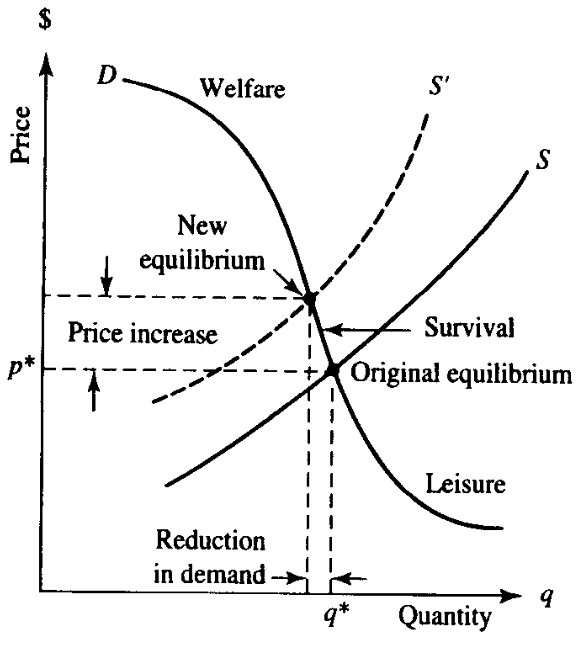
\includegraphics[width=.5\textwidth]{oo.png}
  \end{figure}

\end{frame}

\begin{frame}{继续收税}
  \begin{itemize}
  \item 消费者将付大部分税款
  \item 价格上的巨大震荡是很有可能
  \end{itemize}

  \begin{figure}
    \centering
    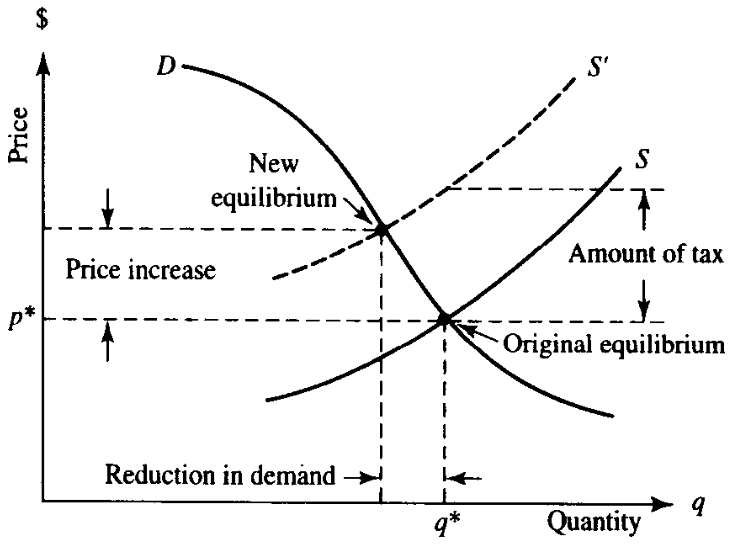
\includegraphics[width=.5\textwidth]{poor.png}
  \end{figure}
  
\end{frame}

\begin{frame}{危机以后}
  \begin{itemize}
  \item 消费者曲线更加平直
  \item 价格对量影响不大
  \end{itemize}

  \begin{figure}
    \centering
    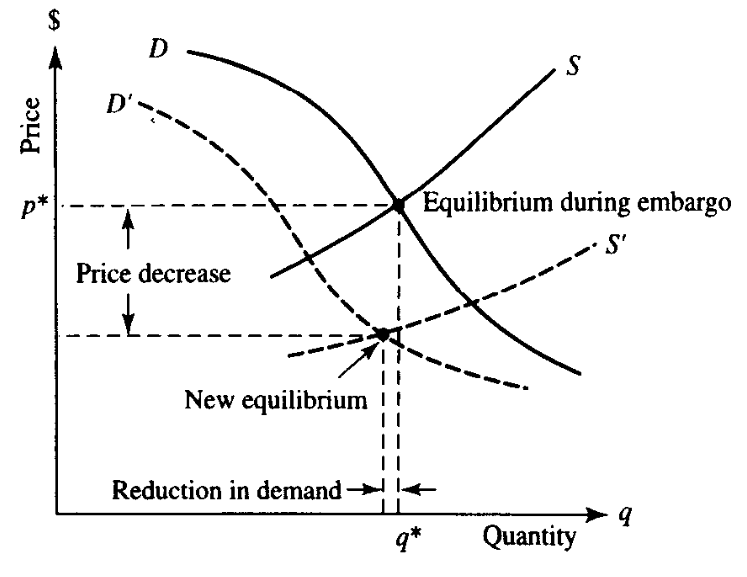
\includegraphics[width=.5\textwidth]{ac.png}
  \end{figure}
  
\end{frame}

\begin{frame}{继续征税}
  \begin{itemize}
  \item 价格变动较少
  \item 石油企业承当大部分税款
  \end{itemize}

  \begin{figure}
    \centering
    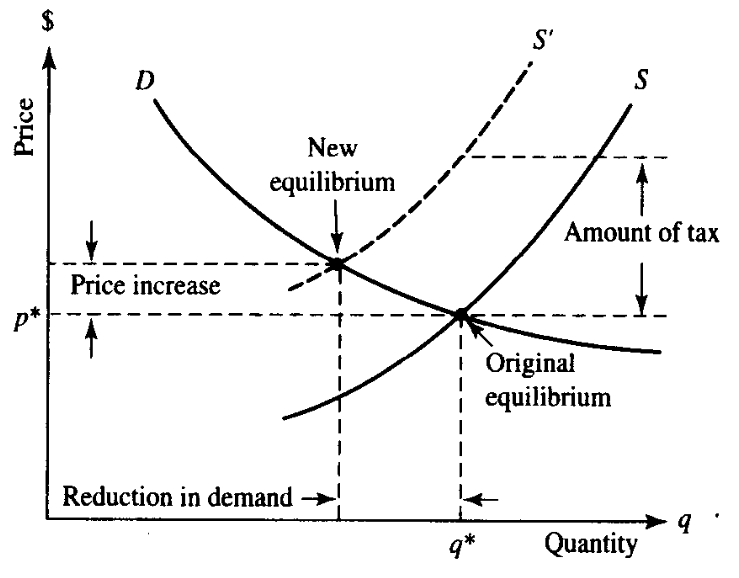
\includegraphics[width=.5\textwidth]{crazy.png}
  \end{figure}

\end{frame}

\begin{frame}
  Questions?
  谢谢!
\end{frame}

\end{document}

%%% Local Variables: 
%%% TeX-master: t
%%% TeX-engine: xetex
%%% End: 
